\documentclass{article}

\usepackage{graphicx}
\usepackage{tikz}
\usepackage{tikzsymbols}
\usetikzlibrary{calc,patterns,shapes.geometric}
\pagestyle{empty}
\usepackage[margin=0pt]{geometry}
\geometry{papersize={14in,12in}}

\def\centerarc[#1](#2)(#3:#4:#5){\draw[#1] ($(#2)+({#5*cos(#3)},{#5*sin(#3)})$) arc (#3:#4:#5);}

\begin{document}
	\begin{figure}
		\centering
		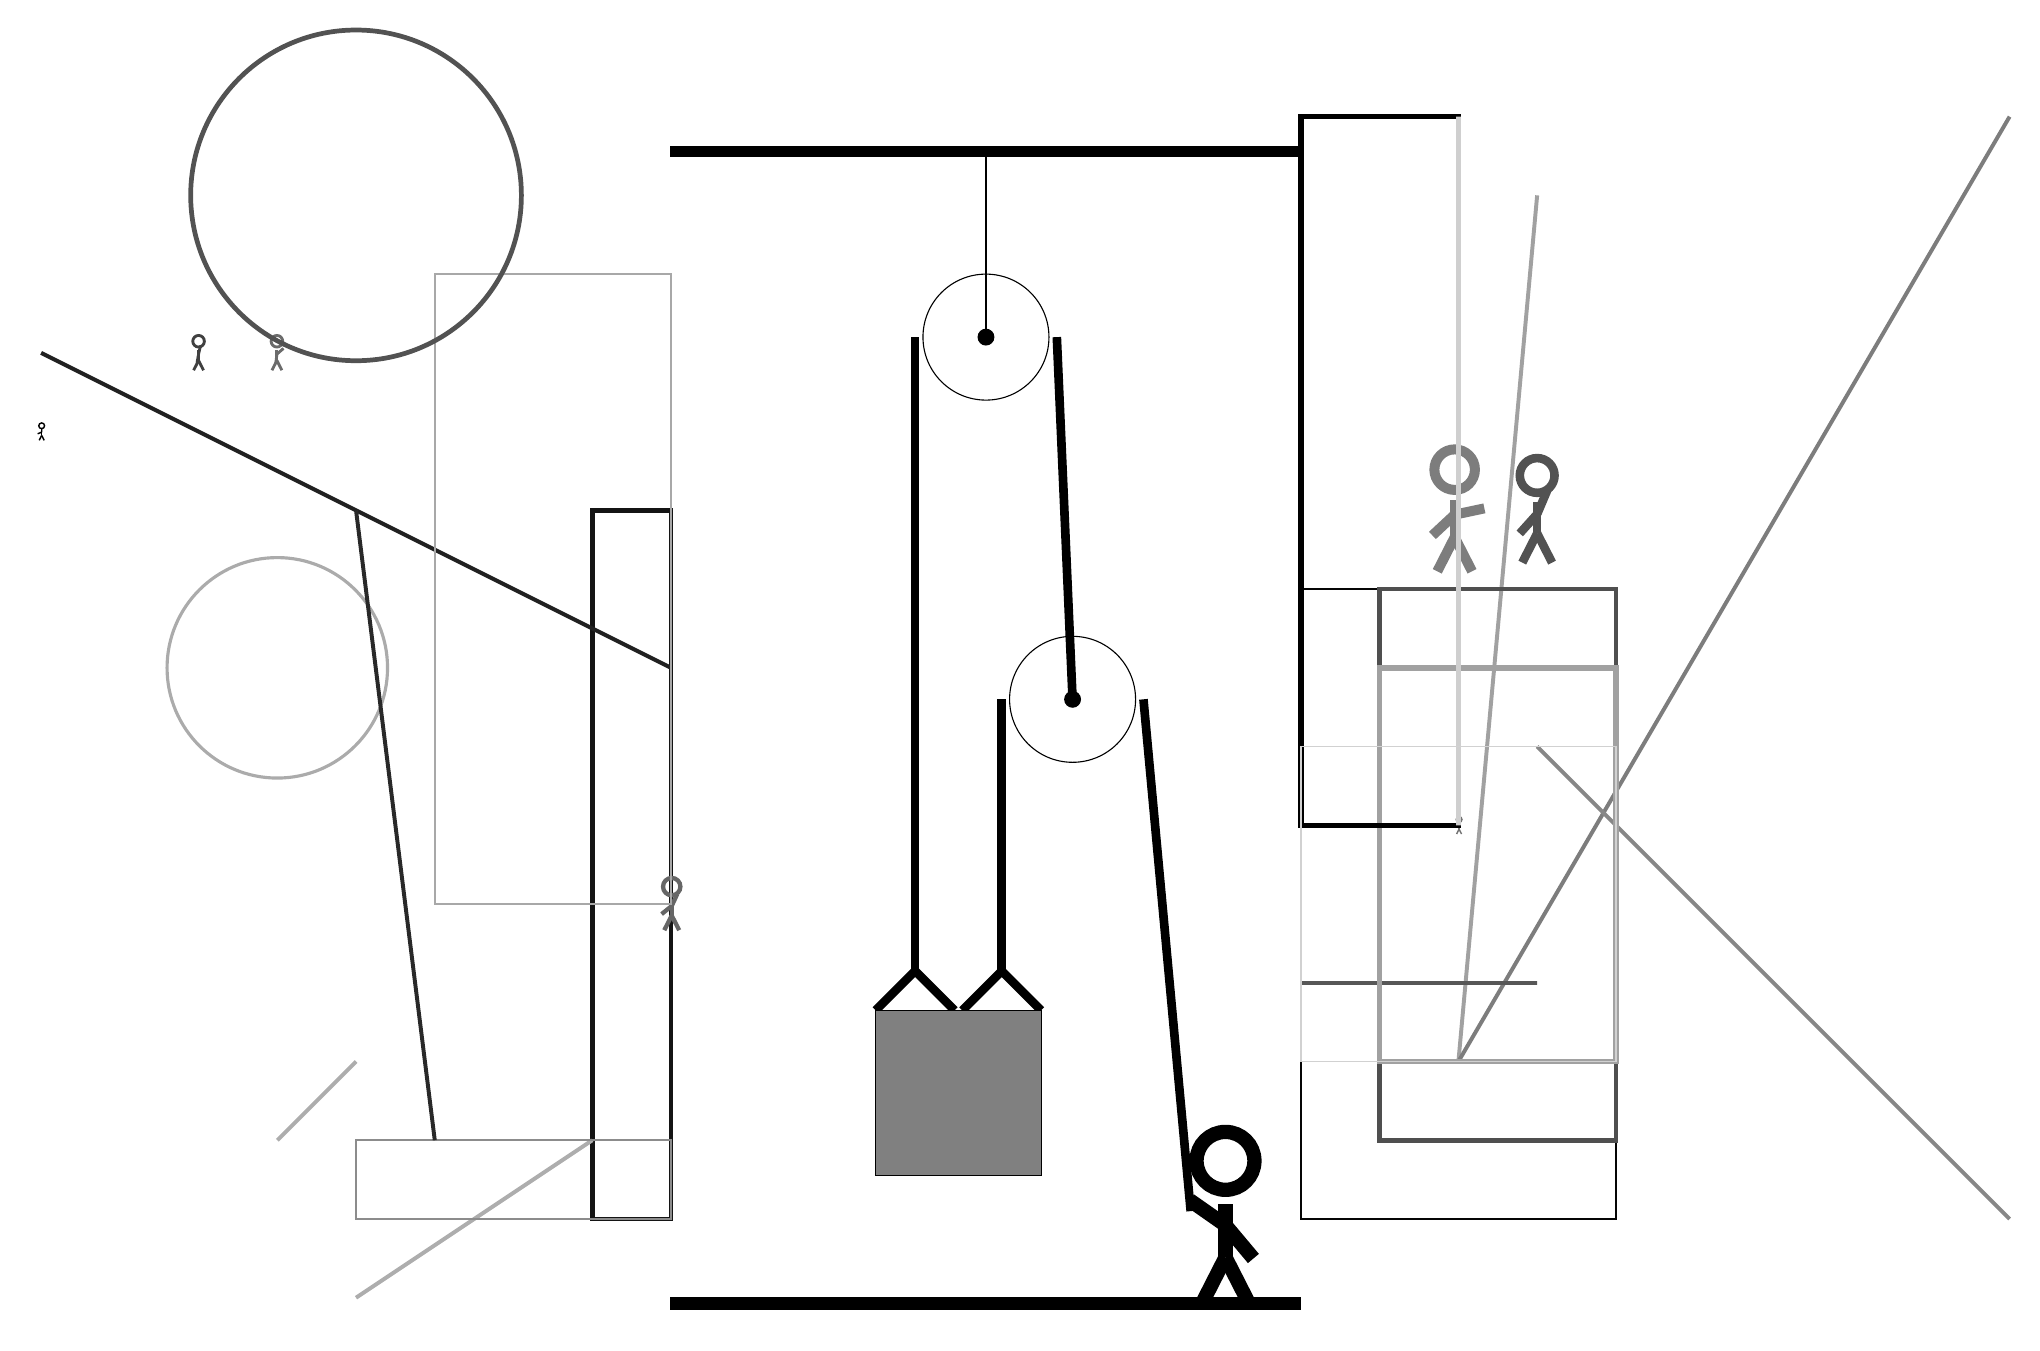
\begin{tikzpicture}
			%%%%% START %%%%%
			
			\draw[fill=black] (-2, 11.5) rectangle (6, 11.625);
			
			\draw (2, 9.2) circle (0.8);
			\draw[fill=black] (2, 9.2) circle (0.1);
			\draw[thick] (2, 9.2) -- (2, 11.5);
			
			\draw[line width=0.3mm, color=black!97] (8, 7) rectangle (8, 10);
			
			\draw[line width=0.6mm, color=black!92] (-2, -2) rectangle (-3, 7);
			\node[line width=0.3mm, color=black!100] at (-10, 8) {\Strichmaxerl[1][21][88]};
			\draw[line width=0.5mm, color=black!37](8, 0) -- (9, 11);
			
			\node[line width=0.6mm, color=black!55] at (8, 3) {\Strichmaxerl[1][12][85]};
			
			\draw[line width=0.5mm, color=black!32](-6, -3) -- (-3, -1);
			
			\draw[line width=0.5mm, color=black!51](8, 0) -- (15, 12);
			\draw[line width=0.3mm, color=black!98] (6, 6) rectangle (10, -2);
			\draw[line width=0.5mm, color=black!47](9, 4) -- (15, -2);
			\draw[line width=0.5mm, color=black!66] (6, 1) rectangle (9, 1);
			\draw[line width=0.6mm, color=black!69] (7, 6) rectangle (10, -1);
			\draw[line width=0.7mm, color=black!37] (7, 0) rectangle (10, 5);
			\node[line width=0.3mm, color=black!58] at (-7, 9) {\Strichmaxerl[2][83][41]};
			
			\draw[line width=0.5mm, color=black!32](-6, 0) -- (-7, -1);
			\draw[line width=0.5mm, color=black!87](-2, 5) -- (-10, 9);
			\node[line width=0.3mm, color=black!68] at (9, 7) {\Strichmaxerl[6][48][67]};
			
			\node[line width=0.5mm, color=black!51] at (8, 7) {\Strichmaxerl[7][43][12]};
			\draw[line width=0.7mm, color=black!100] (6, 12) rectangle (8, 3);
			\node[line width=0.3mm, color=black!75] at (-8, 9) {\Strichmaxerl[2][80][77]};
			
			\node[line width=0.6mm, color=black!60] at (-2, 2) {\Strichmaxerl[3][39][65]};
			\draw[line width=0.2mm, color=black!34] (-2, 2) rectangle (-5, 10);
			
			\draw [line width=0.4mm, color=black!33](-7, 5) circle (1.4);
			\draw[line width=0.6mm, color=black!19] (8, 3) rectangle (8, 12);
			\draw[line width=0.3mm, color=black!45] (-2, -2) rectangle (-6, -1);
			\draw[line width=0.5mm, color=black!84](-6, 7) -- (-5, -1);
			
			\draw[line width=0.2mm, color=black!18] (6, 4) rectangle (10, 0);
			\draw [line width=0.6mm, color=black!68](-6, 11) circle (2.1);
			
			\draw (3.1, 4.6) circle (0.8);
			\draw[fill=black] (3.1, 4.6) circle (0.1);
			
			\draw[line width = 1.1mm]  (0.6, 0.65) -- (1.1, 1.15) -- (1.6, 0.65);
			\draw[line width = 1.1mm]  (1.7, 0.65) -- (2.2, 1.15) -- (2.7, 0.65);
			\draw[fill=black!50] (0.6, 0.65) rectangle (2.7, -1.45);
			
			\draw[line width = 1.1mm] (1.1, 9.2) -- (1.1, 1.15);
			\centerarc[line width = 1.1mm](2, 9.2)(0:180:0.9);
			\draw[line width = 1.1mm] (2.9, 9.2) -- (3.1, 4.6);
			\draw[line width = 1.1mm] (2.2, 4.6) -- (2.2, 1.15);
			\centerarc[line width = 1.1mm](3.1, 4.6)(0:180:0.9);
			\draw[line width = 1.1mm] (4.0, 4.6) -- (4.6, -1.9);
			
			\node at (5, -2) {\Strichmaxerl[10][-35][-50]};
			
			\draw[fill=black] (-2, -3) rectangle (6, -3.15);
			
			%%%%% END %%%%%
		\end{tikzpicture}
	\end{figure}	
\end{document}